%%%%%%%%%%%%%%%%%%%%%%%%%%%%%%%%%%%%%%%%%%%%%%%%%%%%%%%%%%%%%%%%%%%%%%%%%
% Antes de correr el código:
% 1. Ingresar al Menu
% 2. Cambiar la opción "Compiler" a XeLaTeX
% 3. Cambiar la opción "TeX live version" a 2020 (opacidad de la imagen)
%%%%%%%%%%%%%%%%%%%%%%%%%%%%%%%%%%%%%%%%%%%%%%%%%%%%%%%%%%%%%%%%%%%%%%%%%
\documentclass[10pt]{article}
\usepackage[T1]{fontenc}
\usepackage[utf8]{inputenc}
\usepackage[spanish]{babel}
\usepackage{listings}
\lstset{language=R}
\usepackage[a4paper]{geometry}
\usepackage[dvipsnames]{xcolor}
\usepackage[framemethod=TikZ]{mdframed}
\usepackage{graphicx,tikz}
\usepackage{array}

\geometry{top=2.54cm, bottom=2.54cm, left=2.54cm, right=2.54cm}

%\usepackage[sort&compress]{natbib} %Bibliografía
\usepackage{url}
\usepackage{lipsum} 
\usepackage{wrapfig}
\usepackage{subcaption}
\usepackage{multicol}
%==========================================
%======     FUENTE PARA CÓDIGOS      ======
%==========================================
\definecolor{codegreen}{rgb}{0,0.6,0}
\definecolor{codegray}{rgb}{0.1,0.1,0.1}
\definecolor{backcolour}{rgb}{0.98,0.98,0.98}

\lstdefinestyle{mystyle}{
  backgroundcolor=\color{backcolour},   
  commentstyle=\color{codegreen},
  keywordstyle=\color{blue},
  numberstyle=\tiny\color{codegray},
  stringstyle=\color{codegreen},
  basicstyle=\ttfamily\footnotesize,
  breakatwhitespace=false,         
  breaklines=true,                 
  captionpos=b,                    
  keepspaces=true,                 
  numbers=left,                    
  numbersep=5pt,                  
  showspaces=false,                
  showstringspaces=false,
  showtabs=false,                  
  tabsize=2
}

%==========================================
%=======     CUADROS DE TEXTO      ========
%==========================================
\newcounter{theo}[section]\setcounter{theo}{0}
\renewcommand{\thetheo}{\arabic{theo}}
\newenvironment{theo}[2][]{%
\refstepcounter{theo}%
\ifstrempty{#1}%
{\mdfsetup{%
frametitle={%
\tikz[baseline=(current bounding box.east),outer sep=0pt]
\node[anchor=east,rectangle,fill=NavyBlue!50]
{\strut Teorema~\thetheo};}}
}%
{\mdfsetup{%
frametitle={%
\tikz[baseline=(current bounding box.east),outer sep=0pt]
\node[anchor=east,rectangle,fill=NavyBlue!40]
{\strut Teorema~\thetheo:~#1};}}%
}%
\mdfsetup{innertopmargin=5pt,innerbottommargin=10pt,linecolor=NavyBlue!60,%
linewidth=2pt,topline=true,%
frametitleaboveskip=\dimexpr-\ht\strutbox\relax
}
\begin{mdframed}[]\relax%
\label{#2}}{\end{mdframed}}

%==========================================
%==========     ESTILO TITLE     ==========
%==========================================
\newcommand{\City}[1]{\def\City{#1}}
\newcommand{\Cargo}[1]{\def\Cargo{#1}}

\makeatletter         
\renewcommand\maketitle{
\begin{flushleft}
{\textcolor{black}{\Huge \bfseries \@title }}\\[1ex]
\rule{\textwidth}{0.6pt}\\
\end{flushleft}
\vspace{-0.5cm}
\begin{flushright}
{\large \textit {\City, \@date}}\\[4ex]
\end{flushright}

\begin{flushleft}
\textcolor{NavyBlue!80}{{\large  \@author} }\\[1.5ex]
\textcolor{NavyBlue!80}{{\large  \Cargo} }\\[5ex]
\end{flushleft} } % Note the extra }
\makeatother
%

%==========================================
%==========    ESTILO CAPTION    ==========
%==========================================
\usepackage{caption}
\captionsetup[table]{name=Tabla ,textfont={it}, labelfont={bf},
                     justification=centering,
                     width =\dimexpr \textwidth-0.5cm\relax}
\captionsetup[figure]{textfont={it}, labelfont={bf},
                      justification=centering, skip=2pt,
                      belowskip=-5pt}
                      
%==========================================
%==========     ESTILO ITEM      ==========
%==========================================
\renewcommand{\labelitemi}{$\bullet$} 
\renewcommand{\labelitemii}{$\circ$} 
\renewcommand{\labelitemiii}{$\cdot$} 

%==========================================
%===   	LINKS (Agregar Hyperlinks)     ====
%==========================================
%\usepackage[style=apa]{biblatex}
\usepackage[style=apa,
            urldate=long]{biblatex} %bibstyle=authoryear, dejar esta opccion para que se vea el cambio en los parentesis []
\addbibresource{Bib.bib}

% \DeclareFieldFormat{doi}{%
%     DOI\addcolon\space   % <--- doi instead of DOI
%     \ifhyperref
%         {\href{http://doi.org/\detokenize{#1}}{\detokenize{#1}}}
%         \space
% }

\DeclareSourcemap{
  \maps[datatype=bibtex]{
    \map{
      \step[fieldsource=note, final]
      \step[fieldset=addendum, origfieldval, final]
      \step[fieldset=note, null]}
      }
}

% \DeclareFieldFormat{urldate}{\mkbibbrackets{\bibstring{urlseen}\space#1}}
%\DeclareFieldFormat{type}{\mkbibbrackets{\bibstring{}#1}}


\DefineBibliographyStrings{english}{urlseen = {Accessed }    
}

\usepackage[colorlinks=true,linkcolor=RoyalBlue,
            citecolor=RoyalBlue,urlcolor=RoyalBlue]{hyperref}

%==============================================================
%==============================================================
\title{Titulo}
\City{Ciudad}
\date{01 de Enero de 2023}
\author{Nombre y Apellido}
\Cargo{Cargo}
%==============================================================
%==============================================================

%%%%%%%%%%%%%%%%%%%%%%%%%%%%%%%%%%%%%%%%%%%%%%%%%%%%%%%%%%%%%%%
%%%%%%%%%%%%                 INICIO                %%%%%%%%%%%% 
%%%%%%%%%%%%%%%%%%%%%%%%%%%%%%%%%%%%%%%%%%%%%%%%%%%%%%%%%%%%%%%
\begin{document}

\maketitle

\section*{Introducción}
\lipsum[2-3]

\section*{Reporte de error}
Se reportó un error con las siguientes características:

\begin{table}[htp!]
\begin{center}
\begin{tabular}{>{\centering\arraybackslash}m{3cm}| >{\arraybackslash}m{11cm} }
\hline
\\
ID number & 2147483647 \\
\\
\hline
\\
Name & \texttt{321 Error validating request.- 'br':'cause - Invalid account code '1'} \\
\\
\hline
\\
Date & 14/Ene/2023 \\
\\
\hline
\end{tabular}
\end{center}
\end{table}

\subsection*{Descripción}
El error en sí, según algunos foros, puede ser debido al \textbf{TWS} o por una letra de más al final de la \texttt{Account code}

\begin{mdframed}[backgroundcolor=NavyBlue!5,middlelinecolor=MidnightBlue,
                 middlelinewidth=2pt,shadow=false,roundcorner=3pt]
\lipsum[2][1-4]
\end{mdframed}

\newpage

\lipsum[1][1-8]

\begin{wrapfigure}{r}{0.21\textwidth}  
    \centering
    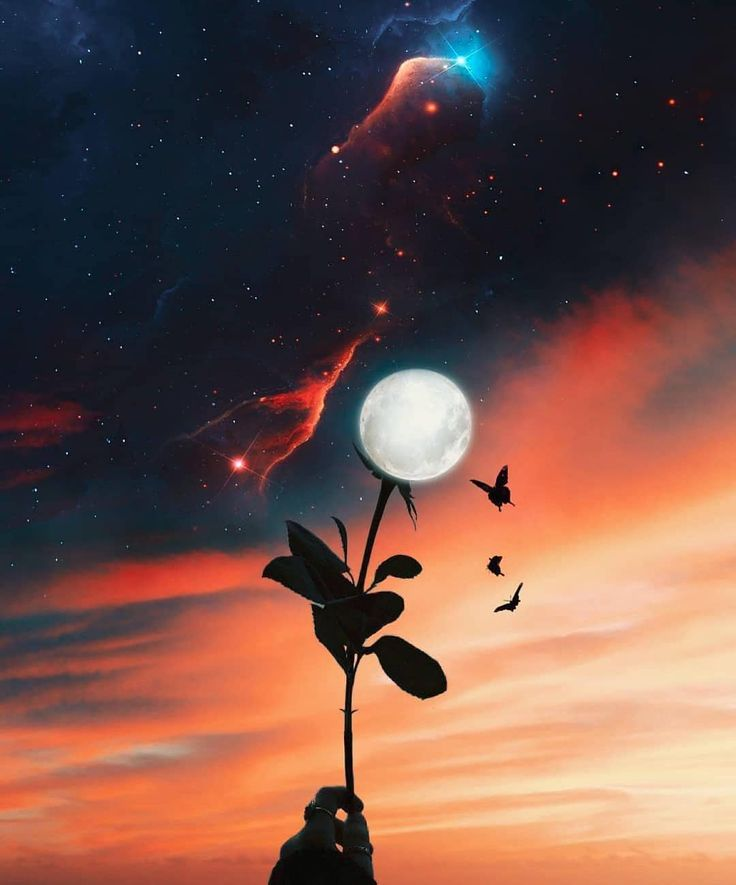
\includegraphics[width=\linewidth]{Imagenes/ImgEj1.jpg} 
    \caption{Caption 1}
    \label{fig:wrapfig}
\end{wrapfigure}

\lipsum[4][1-10]

\lipsum[8]

\lipsum[10][1-6]

\begin{figure}[h!]
    \centering
    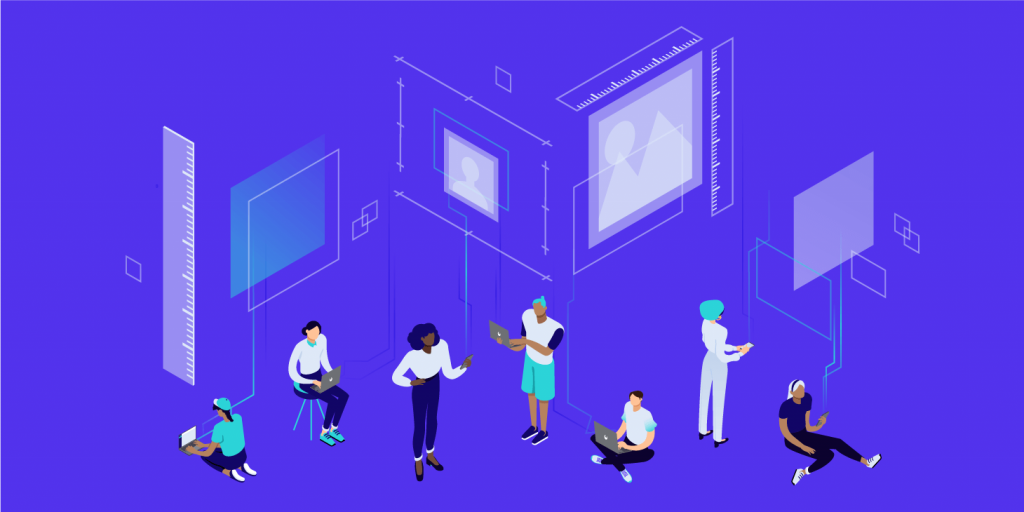
\includegraphics[scale=0.2, angle=4]{Imagenes/ImgEj2.png}
    \caption{Caption}
    \label{fig:my_label}
\end{figure}

\begin{theo}[Pythagoras teorema]{thm:pythagoras}
In a right triangle, the square of the hypotenuse is equal to the sum of the squares of the catheti. $$a^2+b^2=c^2$$
\end{theo}

In mathematics, the Pythagorean theorem, also known as Pythagoras theorem (see theorem \ref{thm:pythagoras}), is a relation in Euclidean geometry among the three sides of a right triangle.


\section*{Motivación}

%%%%%%%%%%%%%%%%%%%%%%%
Esta sección\footnote{A veces esta sección se denomina \textit{justificación}, aunque \textit{motivación} está más extendido. \lipsum[6][1-6]} describe qué factores han hecho al estudiante decantarse por trabajar en éste y no en otro tema. Las imágenes se pueden, y se deben, citar y referenciar. Más aun, cuando se han sacado de internet. En este apartado se hablará de las imágenes extraídas online, que se referencian en estilo de: figuras, imágenes y/o tablas. También se tratarán las imágenes extraídas de redes sociales como Twitter, Instagram o YouTube.
%%%%%%%%%%%%%%%%%%%%%%

\newpage

\begin{figure}[h!]
  \begin{subfigure}{0.5\textwidth}
     \centering
     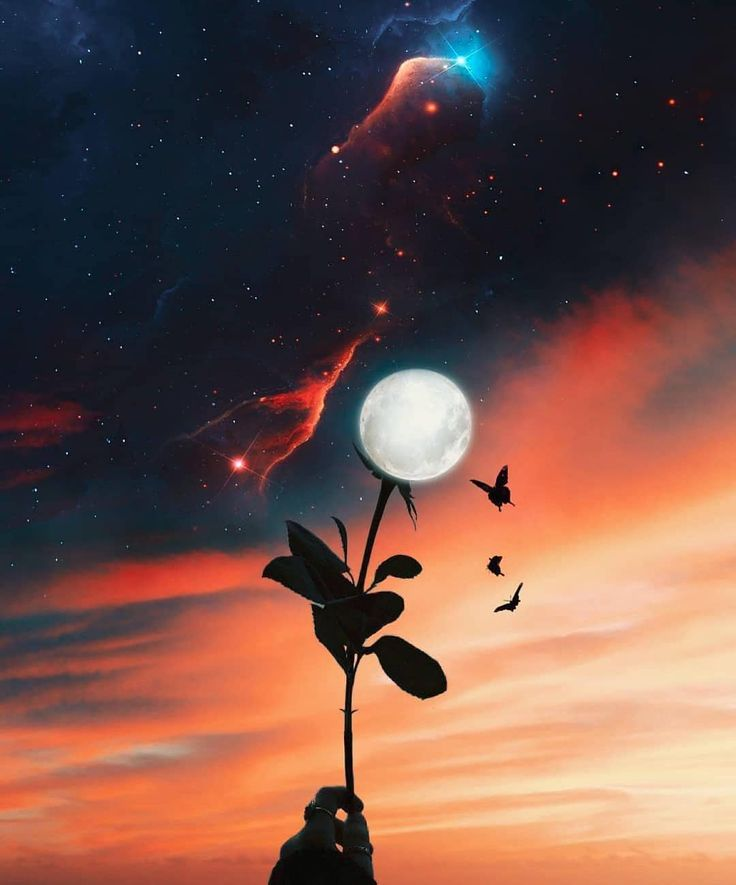
\includegraphics[width=0.6\linewidth]{Imagenes/ImgEj1.jpg} 
     \caption{Caption1}
     \label{fig:subim1}
     \end{subfigure}
  \begin{subfigure}{0.5\textwidth}
     \centering
     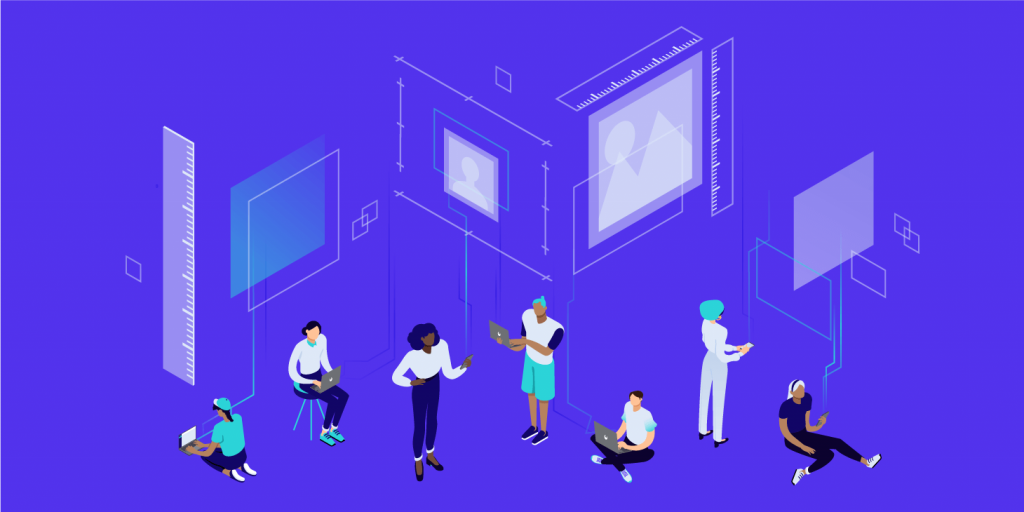
\includegraphics[scale=0.3]{Imagenes/ImgEj2.png}
     \caption{Caption 2}
     \label{fig:subim2}
     \end{subfigure}

  \caption{Caption for this figure with two images}
  \label{fig:image2}
\end{figure}

\lipsum[7]

\begin{table}[h!]
    \centering
    \begin{tabular}{ |p{3cm}||p{3cm}|p{3cm}|p{3cm}|  }
    \hline
    \multicolumn{4}{|c|}{Country List} \\
    \hline
     Country Name or Area Name& ISO ALPHA 2 Code &ISO ALPHA 3 Code&ISO numeric Code\\
    \hline
     Afghanistan   & AF    &AFG&   004\\
     Aland Islands&   AX  & ALA   &248\\
     Albania &AL & ALB&  008\\
     Algeria    &DZ & DZA&  012\\
     American Samoa&   AS  & ASM&016\\
     Andorra& AD  & AND   &020\\
     Angola& AO  & AGO&024\\
    \hline
    \end{tabular}
    \caption{Rows and columns can be merged to create larger table cells. The following example uses the \textit{multicolumn} command to merge several columns: }
    \label{tab:my_label}
\end{table}

\lipsum[9][1-5]


\begin{multicols}{2}
\begin{itemize}
    \item Fedora Versions
    \begin{itemize}
        \item Fedora 8
        \item Fedora 9
        \begin{itemize}
            \item Werewolf
            \item Sulphur
            \begin{itemize}
                \item 2007-05-31
                \item 2008-05-13
            \end{itemize}
        \end{itemize}
    \end{itemize}
    \item Fedora Spin
    \item Fedora Silverblue
\end{itemize}

\columnbreak

% Itemize style
\begin{itemize}
    \item[$\ast$] Asterisk 
    \item[$\diamond$] Diamond 
    \item[$\circ$] Circle 
    \item[$\cdot$] Period
    \item[$\bullet$] Bullet (default)
    \item[--] Dash
    \item[$-$] Another dash
\end{itemize}

\end{multicols}

\newpage

\begin{mdframed}[backgroundcolor=NavyBlue!5,middlelinecolor=MidnightBlue,
                 middlelinewidth=2pt,shadow=false,roundcorner=3pt]
    Vertical farming has 3 main cropping systems:
    \begin{itemize}
        \item size{Aeroponics} This system aims to place the crop is suspended in the air, therefore, irrigation is done by a mist or spray containing the necessary minerals and nutrients, which is supplied directly to the roots.
        \textbf{Hydroponics.} For this, the roots remain submerged in water, or a liquid solution containing the nutrients it requires, plus the water must always be in motion. 
        \textbf{Aquaponics:} The system is similar to the previous one, with the difference that in this one not only plants are cultivated, but also aquatic animals are raised. The animal waste is used as fertilizer for the plants, since the water where the animals live is filtered and irrigated for cultivation. 
    \end{itemize}
    
        \begin{center}
           \captionsetup{type=figure} % <---
           \begin{minipage}{.3\textwidth}
              \subfloat[Aeroponía]{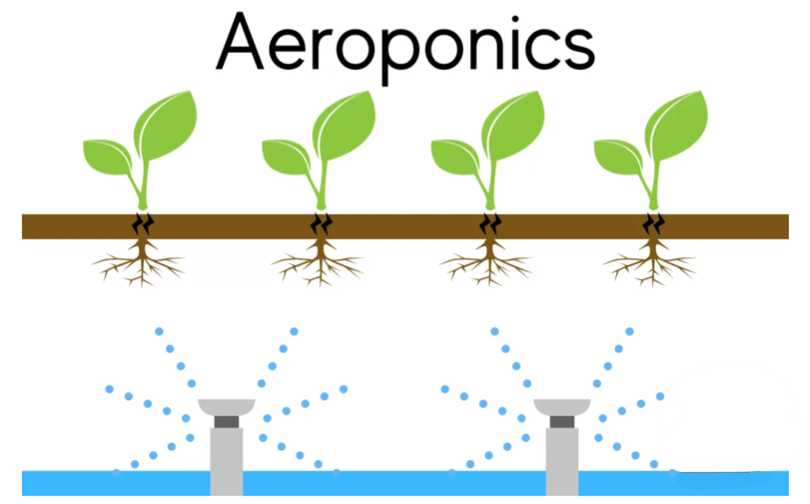
\includegraphics[width=\linewidth]{Imagenes/VfarmAero.png}}
              \label{fig:sub1}
           \end{minipage}%
           \hfill
           \begin{minipage}{.3\textwidth}
              \subfloat[Hidroponía]{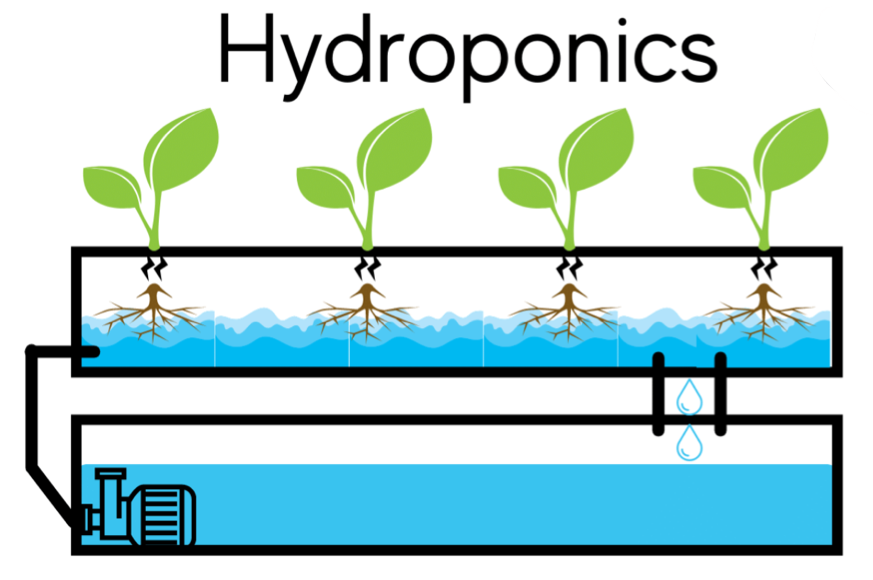
\includegraphics[width=\linewidth]{Imagenes/VfarmHydro.png}}
              \label{fig:sub2}
           \end{minipage}
           \hfill
           \begin{minipage}{.3\textwidth}
              \subfloat[Acuaponía]{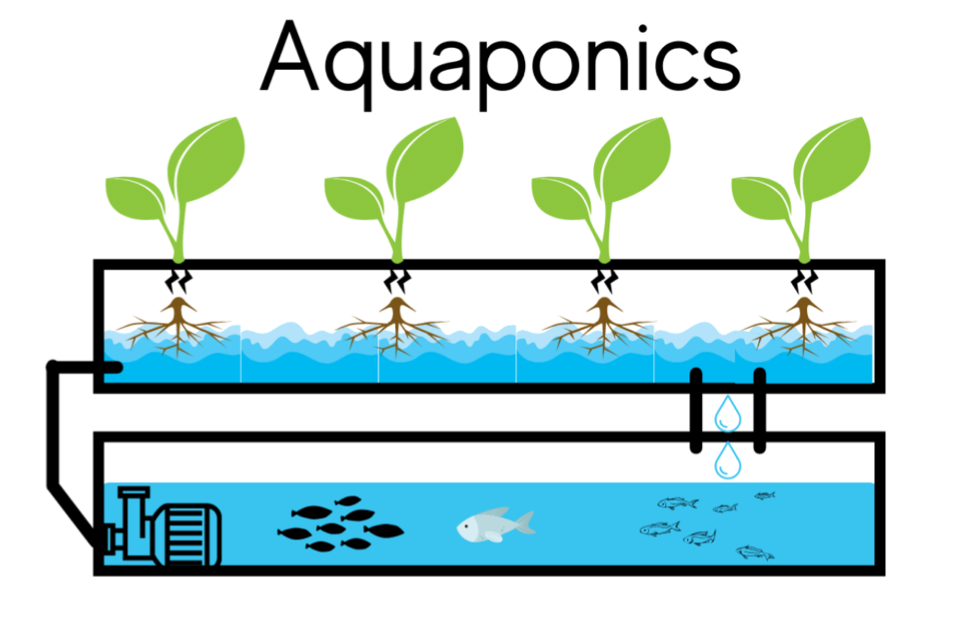
\includegraphics[width=\linewidth]{Imagenes/VfarmAqua.png}}
              \label{fig:sub2}
           \end{minipage}

           \captionof{figure}{Tipos de cultivo en agricultira vertical}
           \label{fig:test}
        \end{center}
        
    \end{mdframed}

    Another of this company's strengths is LED lighting. AeroFarms has focused on specialized lighting software, where the algorithm is customized for each plant, providing them with exactly the spectrum, intensity and frequency of light they need for photosynthesis. With this set of lights, the size, shape, texture, color, flavor and even nutrients of the plants can be optimized. (\cite{AeroFarm2})
    
\section*{Vertical farming in small experiments:}

The following are articles that explain, on a small scale, how a vertical farming design can be implemented:

\begin{itemize}
    \item \textit{''Artificial Intelligence Driven Vertical Farming Management System"} (\url{https://www.iaeng.org/publication/WCE2022/WCE2022_pp108-113.pdf})
     \item \textit{''Combining an R-Based Evolutionary Algorithm and Hydrological Model for Effective Parameter Calibration "} (\url{https://www.mdpi.com/2073-4441/10/10/1339})
     \item \textit{"Nutrient Use in Vertical Farming: Optimal Electrical Conductivity of Nutrient Solution for Growth of Lettuce and Basil in Hydroponic Cultivation"} (\url{https://www.researchgate.net/publication/354339414})
     \item \textit{"Vertical Farming Case Study, Published by Alberta Agriculture, Forestry and Rural Economic Developmen"} (\url{https://open.alberta.ca/dataset/1c1f48a2-63b9-4dcb-823c-aa49a9a7c810/resource/b0cdfe26-7058-4ee9-a40a-7a3dcff2fe89/download/af-vertical-farming-case-study-2021-04.pdf})
\end{itemize}


%==============================================================

\newpage
\section*{Referencias}
  \nocite{*}
  \printbibliography[heading=none]

\end{document}

